% Important: If latex complains about unicode characters,
% please use "\usepackage[utf8x]{inputenc}" in your preamble
% You can change the size of the picture by putting it into the construct:
% 1) \resizebox{10cm}{!}{"below picture"} to scale horizontally to 10 cm
% 2) \resizebox{!}{15cm}{"below picture"} to scale vertically to 15 cm
% 3) \resizebox{10cm}{15cm}{"below picture"} a combination of above two
% It is not recomended to use the scale option of the tikzpicture environment.
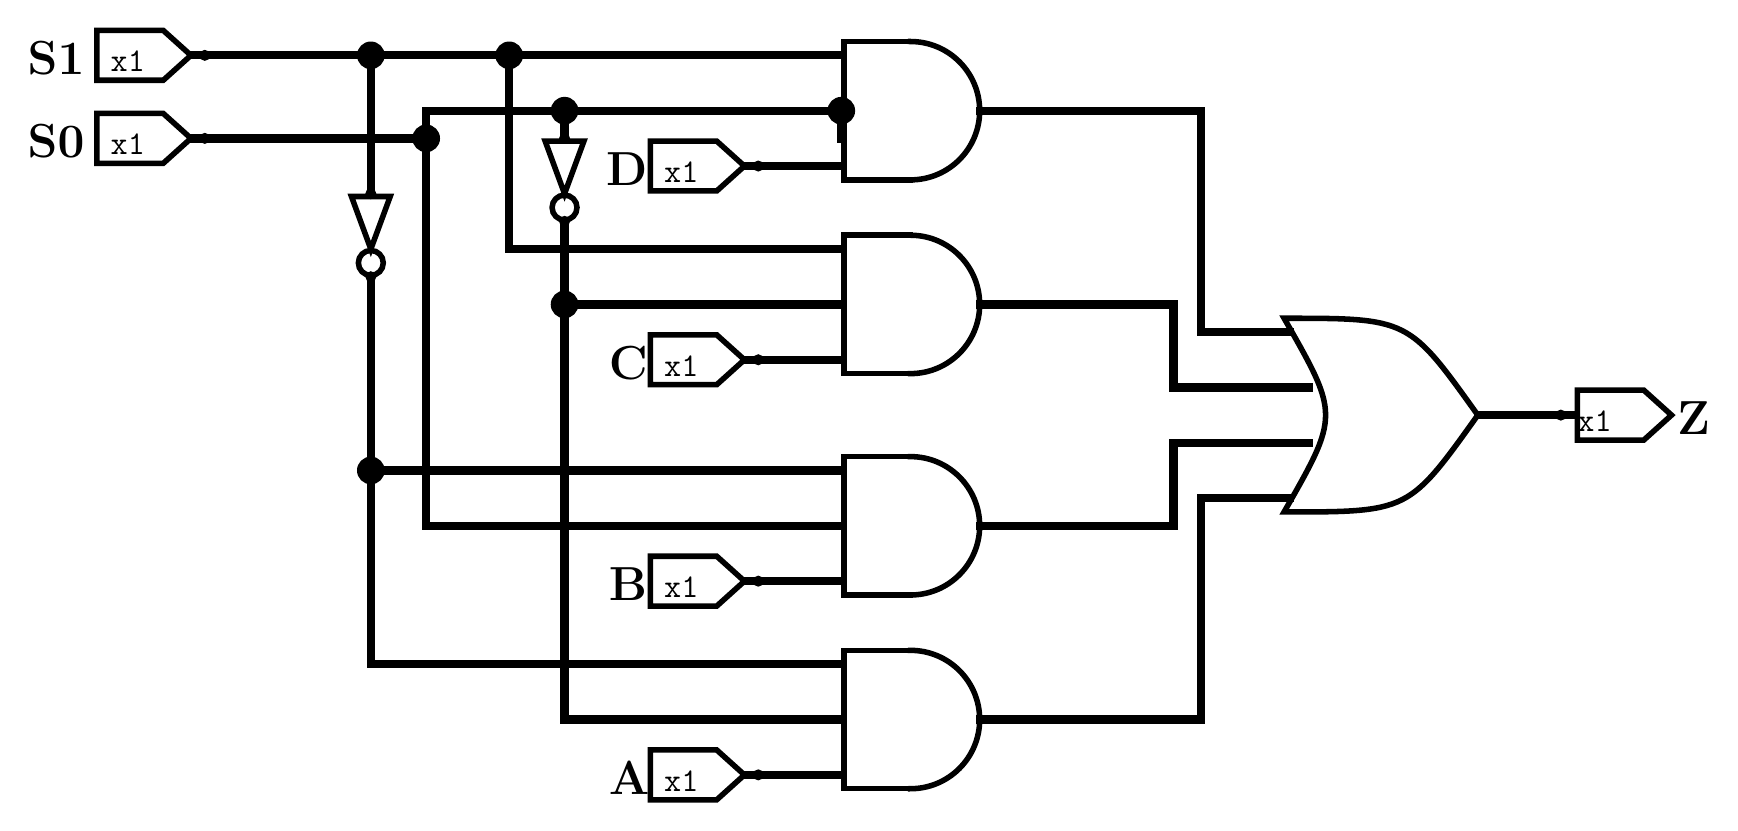
\begin{tikzpicture}[x=1pt,y=-1pt,line cap=rect]
\def\logisimfontA#1{\fontfamily{cmr}{#1}} % Replaced by logisim, original font was "SansSerif"
\def\logisimfontB#1{\fontfamily{cmtt}{#1}} % Replaced by logisim, original font was "Monospaced"
\definecolor{custcol_0_0_0}{RGB}{0, 0, 0}
\definecolor{custcol_ff_ff_ff}{RGB}{255, 255, 255}
\draw [line width=3.0pt, custcol_0_0_0 ]  (179.0,15.0) -- (299.0,15.0) ;
\draw [line width=3.0pt, custcol_0_0_0 ]  (129.0,95.0) -- (129.0,165.0) -- (129.0,235.0) -- (299.0,235.0) ;
\draw [line width=3.0pt, custcol_0_0_0 ]  (129.0,165.0) -- (299.0,165.0) ;
\draw [line width=3.0pt, custcol_0_0_0 ]  (199.0,35.0) -- (299.0,35.0) -- (299.0,45.0) ;
\draw [line width=3.0pt, custcol_0_0_0 ]  (299.0,255.0) -- (199.0,255.0) -- (199.0,105.0) -- (299.0,105.0) ;
\draw [line width=3.0pt, custcol_0_0_0 ]  (199.0,75.0) -- (199.0,105.0) ;
\draw [line width=3.0pt, custcol_0_0_0 ]  (529.0,145.0) -- (559.0,145.0) ;
\draw [line width=3.0pt, custcol_0_0_0 ]  (199.0,45.0) -- (199.0,35.0) -- (149.0,35.0) -- (149.0,45.0) -- (149.0,185.0) -- (299.0,185.0) ;
\draw [line width=3.0pt, custcol_0_0_0 ]  (129.0,15.0) -- (129.0,65.0) ;
\fill [line width=3.0pt, custcol_0_0_0]  (299.0,35.0) ellipse (5.0 and 5.0 );
\fill [line width=3.0pt, custcol_0_0_0]  (199.0,105.0) ellipse (5.0 and 5.0 );
\fill [line width=3.0pt, custcol_0_0_0]  (129.0,15.0) ellipse (5.0 and 5.0 );
\fill [line width=3.0pt, custcol_0_0_0]  (149.0,45.0) ellipse (5.0 and 5.0 );
\fill [line width=3.0pt, custcol_0_0_0]  (199.0,35.0) ellipse (5.0 and 5.0 );
\fill [line width=3.0pt, custcol_0_0_0]  (179.0,15.0) ellipse (5.0 and 5.0 );
\fill [line width=3.0pt, custcol_0_0_0]  (129.0,165.0) ellipse (5.0 and 5.0 );
\draw [line width=2.0pt, custcol_0_0_0] (324.0,60.0) arc (90.0:-90.0:25.0 and 25.0 );
\draw [line width=2.0pt, custcol_0_0_0 ]  (324.0,10.0) -- (300.0,10.0) -- (300.0,60.0) -- (324.0,60.0) ;
\draw [line width=3.0pt, custcol_0_0_0 ]  (349.0,35.0) -- (429.0,35.0) -- (429.0,115.0) -- (459.0,115.0) -- (461.0,115.0) ;
\draw [line width=3.0pt, custcol_0_0_0 ]  (349.0,105.0) -- (419.0,105.0) -- (419.0,135.0) -- (459.0,135.0) -- (468.0,135.0) ;
\draw [line width=3.0pt, custcol_0_0_0 ]  (349.0,185.0) -- (419.0,185.0) -- (419.0,155.0) -- (459.0,155.0) -- (468.0,155.0) ;
\draw [line width=3.0pt, custcol_0_0_0 ]  (349.0,255.0) -- (429.0,255.0) -- (429.0,175.0) -- (459.0,175.0) -- (461.0,175.0) ;
\draw [line width=2.0pt, custcol_0_0_0 ]  (529.0,145.0) .. controls  (504.0,110.0)  ..  (459.0,110.0) .. controls  (479.0,145.0)  ..  (459.0,180.0) .. controls  (504.0,180.0)  ..  (529.0,145.0) -- cycle ;
\draw [line width=2.0pt, custcol_0_0_0] (324.0,210.0) arc (90.0:-90.0:25.0 and 25.0 );
\draw [line width=2.0pt, custcol_0_0_0 ]  (324.0,160.0) -- (300.0,160.0) -- (300.0,210.0) -- (324.0,210.0) ;
\draw [line width=2.0pt, custcol_0_0_0] (324.0,130.0) arc (90.0:-90.0:25.0 and 25.0 );
\draw [line width=2.0pt, custcol_0_0_0 ]  (324.0,80.0) -- (300.0,80.0) -- (300.0,130.0) -- (324.0,130.0) ;
\draw [line width=2.0pt, custcol_0_0_0] (324.0,280.0) arc (90.0:-90.0:25.0 and 25.0 );
\draw [line width=2.0pt, custcol_0_0_0 ]  (324.0,230.0) -- (300.0,230.0) -- (300.0,280.0) -- (324.0,280.0) ;
\draw [line width=3.0pt, custcol_0_0_0 ]  (264.0,55.0) -- (269.0,55.0) -- (299.0,55.0) ;
\draw [line width=2.0pt, custcol_0_0_0 ]  (254.0,64.0) -- (264.0,55.0) -- (254.0,46.0) -- (230.0,46.0) -- (230.0,64.0) -- cycle;
\logisimfontB{\fontsize{12pt}{12pt}\selectfont\node[inner sep=0, outer sep=0, custcol_0_0_0, anchor=base west] at  (235.0,61.0)  {x1};}
\logisimfontA{\fontsize{16pt}{16pt}\fontseries{bx}\selectfont\node[inner sep=0, outer sep=0, custcol_0_0_0, anchor=base west] at  (214.0,62.0)  {D};}
\fill [line width=2.0pt, custcol_0_0_0]  (269.0,55.0) ellipse (2.0 and 2.0 );
\draw [line width=3.0pt, custcol_0_0_0 ]  (264.0,125.0) -- (269.0,125.0) -- (299.0,125.0) ;
\draw [line width=2.0pt, custcol_0_0_0 ]  (254.0,134.0) -- (264.0,125.0) -- (254.0,116.0) -- (230.0,116.0) -- (230.0,134.0) -- cycle;
\logisimfontB{\fontsize{12pt}{12pt}\selectfont\node[inner sep=0, outer sep=0, custcol_0_0_0, anchor=base west] at  (235.0,131.0)  {x1};}
\logisimfontA{\fontsize{16pt}{16pt}\fontseries{bx}\selectfont\node[inner sep=0, outer sep=0, custcol_0_0_0, anchor=base west] at  (215.0,132.0)  {C};}
\fill [line width=2.0pt, custcol_0_0_0]  (269.0,125.0) ellipse (2.0 and 2.0 );
\draw [line width=3.0pt, custcol_0_0_0 ]  (264.0,205.0) -- (269.0,205.0) -- (299.0,205.0) ;
\draw [line width=2.0pt, custcol_0_0_0 ]  (254.0,214.0) -- (264.0,205.0) -- (254.0,196.0) -- (230.0,196.0) -- (230.0,214.0) -- cycle;
\logisimfontB{\fontsize{12pt}{12pt}\selectfont\node[inner sep=0, outer sep=0, custcol_0_0_0, anchor=base west] at  (235.0,211.0)  {x1};}
\logisimfontA{\fontsize{16pt}{16pt}\fontseries{bx}\selectfont\node[inner sep=0, outer sep=0, custcol_0_0_0, anchor=base west] at  (215.0,212.0)  {B};}
\fill [line width=2.0pt, custcol_0_0_0]  (269.0,205.0) ellipse (2.0 and 2.0 );
\draw [line width=3.0pt, custcol_0_0_0 ]  (264.0,275.0) -- (269.0,275.0) -- (299.0,275.0) ;
\draw [line width=2.0pt, custcol_0_0_0 ]  (254.0,284.0) -- (264.0,275.0) -- (254.0,266.0) -- (230.0,266.0) -- (230.0,284.0) -- cycle;
\logisimfontB{\fontsize{12pt}{12pt}\selectfont\node[inner sep=0, outer sep=0, custcol_0_0_0, anchor=base west] at  (235.0,281.0)  {x1};}
\logisimfontA{\fontsize{16pt}{16pt}\fontseries{bx}\selectfont\node[inner sep=0, outer sep=0, custcol_0_0_0, anchor=base west] at  (215.0,282.0)  {A};}
\fill [line width=2.0pt, custcol_0_0_0]  (269.0,275.0) ellipse (2.0 and 2.0 );
\draw [line width=2.0pt, custcol_0_0_0 ]  (129.0,85.0) -- (136.0,66.0) -- (122.0,66.0) -- cycle;
\draw [line width=2.0pt, custcol_0_0_0, rotate around={-270: (129.0,90.0) }]  (129.0,90.0) ellipse (4.5 and 4.5 );
\fill [line width=2.0pt, custcol_0_0_0]  (129.0,95.0) ellipse (2.0 and 2.0 );
\fill [line width=2.0pt, custcol_0_0_0]  (129.0,65.0) ellipse (2.0 and 2.0 );
\draw [line width=2.0pt, custcol_0_0_0 ]  (199.0,65.0) -- (206.0,46.0) -- (192.0,46.0) -- cycle;
\draw [line width=2.0pt, custcol_0_0_0, rotate around={-270: (199.0,70.0) }]  (199.0,70.0) ellipse (4.5 and 4.5 );
\fill [line width=2.0pt, custcol_0_0_0]  (199.0,75.0) ellipse (2.0 and 2.0 );
\fill [line width=2.0pt, custcol_0_0_0]  (199.0,45.0) ellipse (2.0 and 2.0 );
\draw [line width=3.0pt, custcol_0_0_0 ]  (563.0,145.0) -- (560.0,145.0) ;
\draw [line width=2.0pt, custcol_0_0_0 ]  (589.0,136.0) -- (599.0,145.0) -- (589.0,154.0) -- (565.0,154.0) -- (565.0,136.0) -- cycle;
\logisimfontB{\fontsize{12pt}{12pt}\selectfont\node[inner sep=0, outer sep=0, custcol_0_0_0, anchor=base west] at  (565.0,151.0)  {x1};}
\logisimfontA{\fontsize{16pt}{16pt}\fontseries{bx}\selectfont\node[inner sep=0, outer sep=0, custcol_0_0_0, anchor=base west] at  (601.0,152.0)  {Z};}
\fill [line width=2.0pt, custcol_0_0_0]  (559.0,145.0) ellipse (2.0 and 2.0 );
\draw [line width=3.0pt, custcol_0_0_0 ]  (64.0,15.0) -- (69.0,15.0) -- (129.0,15.0) -- (179.0,15.0) -- (179.0,85.0) -- (299.0,85.0) ;
\draw [line width=2.0pt, custcol_0_0_0 ]  (54.0,24.0) -- (64.0,15.0) -- (54.0,6.0) -- (30.0,6.0) -- (30.0,24.0) -- cycle;
\logisimfontB{\fontsize{12pt}{12pt}\selectfont\node[inner sep=0, outer sep=0, custcol_0_0_0, anchor=base west] at  (35.0,21.0)  {x1};}
\logisimfontA{\fontsize{16pt}{16pt}\fontseries{bx}\selectfont\node[inner sep=0, outer sep=0, custcol_0_0_0, anchor=base west] at  (5.0,22.0)  {S1};}
\fill [line width=2.0pt, custcol_0_0_0]  (69.0,15.0) ellipse (2.0 and 2.0 );
\draw [line width=3.0pt, custcol_0_0_0 ]  (64.0,45.0) -- (69.0,45.0) -- (149.0,45.0) ;
\draw [line width=2.0pt, custcol_0_0_0 ]  (54.0,54.0) -- (64.0,45.0) -- (54.0,36.0) -- (30.0,36.0) -- (30.0,54.0) -- cycle;
\logisimfontB{\fontsize{12pt}{12pt}\selectfont\node[inner sep=0, outer sep=0, custcol_0_0_0, anchor=base west] at  (35.0,51.0)  {x1};}
\logisimfontA{\fontsize{16pt}{16pt}\fontseries{bx}\selectfont\node[inner sep=0, outer sep=0, custcol_0_0_0, anchor=base west] at  (5.0,52.0)  {S0};}
\fill [line width=2.0pt, custcol_0_0_0]  (69.0,45.0) ellipse (2.0 and 2.0 );
\end{tikzpicture}

